\chapter{Background}

% Introduce what is planning under uncertainty
Planning and reasoning under uncertainty is central to robotic and artificial intelligence research and has 
been an active area of research for decades. It is an umbrella term which touches a
wide spectrum of fields: \textit{economics}, \textit{psychology}, \textit{cognitive science}, \textit{neuroscience},
\textit{robotics} and \textit{artificial intelligence}. The work in this thesis relies on results  and assumptions 
made in cognitive and neuroscience with respect to our beliefs and how we act given them. We complement 
these results by introducing them in a new light to the field of robotics and demonstrate how the human reasoning and belief system 
can be used in situations where the state space is partially observable. The second main theme our work builds on is 
state space estimation. The third component acting given uncertainty in robotics. We make use of results from all 
three fields. We provide a background overview of acting under uncertainty and situate our work within the state of the 
art.

This chapter unfolds as follows: 



\section{Decisions under Uncertainty}
% What is the the reasoning under uncertainty planning problem
% What are all the assumptions which can be made regading the belief

In this section we introduce and frame the problem we seek to solve in generic 
terms. We are concerned with finding a sequence of actions which will lead to the successful 
outcome of a problem being considered; this is the most generic definition. 

There are two key attributes which can make this problem difficult: stochastic actions and latent states. Stochastic 
actions, when applied in the same state will not always result int the same outcome. This type of uncertainty 
can arise from many sources; the outcome of chaotic actions are impossible to predict with certainty, 
think of throwing a die or flipping a coin; In outdoor robotics the terrain might lead to slippage, causing 
the robot to skid or underwater currents might drastically offset the position of an UAV; In articulated 
robots the friction between joints can accumulate to a large error in the end-effector position (especially true 
for cable driven robots). 
The second source of uncertainty is when the underlying state is partially known, in the sense that we do not 
have all the necessary information to reliably determine the state beyond reasonable doubt. In robotics this 
uncertainty can arise from inadequate or noisy sensors. If the environmental conditions in which the robot 
is located is humid, misty or dark. It can make it difficult for the robot to ascertain its position and 
to plan how to achieve a given objective.

The uncertainty of the state and actions have to be quantified. The predominant approach 
is to  represent them by probabilities. For instance the application of a forward action (for a wheeled robot) 
will result in a new position further ahead and a position to the right (due to slippage) with some probability.
An observation through the robots sensors will result in probability distribution over the robots probable location.
Given this quantification of action and observation uncertainty in terms of a probability distribution over the state, 
the agent must now take actions towards accomplishing its goal. To take a decision the agent must assign a utility 
to the outcome of his actions. The utility is to indicate a preference over the outcomes and when combined with 
probabilities leads to decision theory. 

\subsection{Decision theory}

The central question of decision theory is; \textit{how do we take decisions when faced with uncertain outcomes ?} To answer
such a question we need to ground the attributes which are involved when we take a decision, namely our \textbf{beliefs} and 
\textbf{desires}. Beliefs reflect a degree of knowledge we have about the world in which the degree is ascertained by 
the amount of evidence we have in support of our beliefs. Epistemology studies in great detail the relationship between 
truth, beliefs and knowledge. We will not go into a philosophical discussion of their interplay, but make use of the following; 
if we have sufficient evidence in support of our beliefs and they represent the truth then we consider them to 
be a \textbf{rational belief}. As for desires they are linked to our disposition to take action to achieve them; for 
example if I want to switch of my alarm clock I have to look for it in the last area I believed it to be. 
These two attributes, beliefs and desires, are used to frame a decision problem. Early work in decision theory assumed 
that the problem was well grounded and focused on finding what are the \textbf{rational choices} to take given our beliefs 
to achieve our desires. 

\begin{figure}[h]
 \centering
 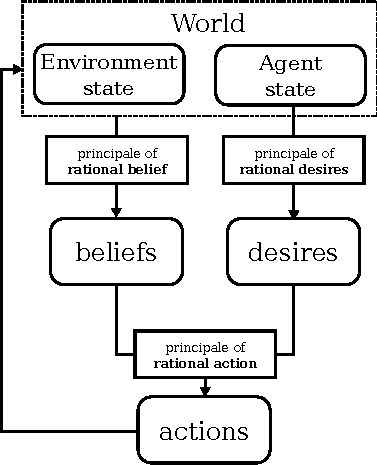
\includegraphics[width=0.5\textwidth]{/home/guillaume/Documents/Thesis/ch2-Background/Figures/cognitive_loop.pdf}
  \caption{ad}
\end{figure}

Early interest in such questions were typically centred around economics such as deciding what should be an appropriate 
investment or wager for a particular gamble. It was noted that the expected monitory outcome of a gamble as a mean of basing a 
decision, would often lead to a course of action which contradicts common sense; a famous example is the St. Petersburg paradox.
In this paradox a bookmaker proposes you the following gamble. An initial pot starts with a content of 2\pounds, the bookmaker proceeds 
to flip a fair coin until the first appearance of a tails which ends the game. Until the occurrence of the first tails 
the money in the pot doubles after every toss. Once the game ends you leave with the content of the pot. As an avid gambler 
and expected value maximiser how much would you be willing to pay to enter this gamble ? A value maximiser would computed 
the expected monetary outcome. The amount of money increases by $2^{n}\pounds$, where $n$ is the number of non-final tosses and 
and the probability of reaching $n$ is $1/2^{n}$. In this case the expected monitory outcome is an infinite number,

\begin{equation*}
\displaystyle \mathop{\mathbb{E}}_{p(n)}\{\pounds\} = \underbrace{\frac{1}{2} 2 \pounds}_{\textrm{first toss}} + \frac{1}{4} 4 \pounds + \dots = \sum\limits_{n=1}^{\infty} 
\frac{2^{n}}{2^{n}}\pounds = \infty \pounds 
\end{equation*}

So your expected gain or return for paying to enter such game is an infinite amount of money, so in principal if you were
seeking to maximise your expected return value you would be willing to pay an amount close to infinity. This does not 
seem a good decision rule; no person in the world would be willing to pay more than $1\pounds$ to enter such game.

Nicola Bernoulli proposed a solution to the problem (later published by his brother Daniel  (\cite{Bernoulli1954})) by introducing the notion 
of a \textbf{utility function}, and he claimed that people should base their decision on the expected utility instead 
of solely the monetary outcomes of a gamble.

\begin{quote}
  \onehalfspacing% <--- Local line spacing
  ``...the value of an item must not be based on its price, but rather on the utility it yields."\par\raggedleft--- \textup{Daniel Bernoulli}
\end{quote}

The introduction of a utility function takes into account that the net worth of a person will influence their decision since 
different people (in terms of their monetary worth) will weigh the gain differently. The utility function introduced by Bernoulli 
was the logarithm of the monetary outcome $x \in X$ weighted by their probability $p(x)$ which results in an expected utility, 

\begin{equation*}\label{eq:exp_utility}
  U(x) = \displaystyle \mathop{\mathbb{E}}_{p(x)} \{ u(x) \} = \sum_{x\in X} p(x) \underbrace{\log(x)}_{u(x)}
\end{equation*}

Different utility functions characterise different levels of risk. When the it is concave as it for Bernoulli's utility function
the person will be \textbf{risk-averse}, when linear \textbf{risk-neural} and convex \textbf{risk-seeking}. 
This was the first introduction of a utility function.

It is later in 1944 that von Neumann and Morgenstern (\cite{VonNeumann1944}) axiomised Bernoulli's utility function 
and proved that if a decision maker has a preference over a set of lotteries\footnote{the term lottery refers 
to a probability distribution in the original text.} which satisfy four axioms
(completeness, transitivity, continuity, independence) then there exists a utility function who's expectation 
preserves this preference. An agent whose decisions can be shown to maximise the vNM expected utility are said 
to be \textbf{rational} and otherwise \textbf{irrational}.  This is the theoretical basis of most economic theory,
it is a \textbf{normative} model of how people should behave given uncertainty. It is also the basis of most 
if not all decision making, cogitative architectures and control policies in AI and robotics 
(to the best of the authors knowledge).

An aspect to keep in mind regarding the vNM model is that it is normative; it states what should be a rational decision 
or behaviour. As a result it is not always consistent with human behaviour. There is great debate regarding 
the predictions made by vNM models with respect to ours. There have been many studies both demonstrating divergence 
between the models predictions and our observed behaviour but also supporting evidence that it does reflect 
the output of our decision making process. Reasons for divergence have been attributed to the way we 
weigh probabilities and how the decision problem is framed. But probably the most important aspect is that 
in most decisions we are faced with the quantification and rationality of our beliefs might not be adequate
and limitations of our working memory will come into play in the final decision.

Nevertheless vNM agents are predominantly used in AI and robotics as a means of implementing 
a decision making process or a control policy. In psychology and cogitative science vNM agents
are a used for comparing human behaviour against an optimal strategy (by optimal we mean it is rational in 
the vNM sense). 

%(see prescriptive models(\cite{Kahneman79prospecttheory}). 

% vNM is concerned with a one shot only decision, but what if we have to take a sequence of decisions ? What 
% happens then ?

%How is the uncertainty quantified ? Answer: probability theory
%How does the agent make a decision ? He must assigned a preference to the outcome of various actions
%Utility theory and combined with probability lead to decision theory.

% Speak about the historical context of plannig un
% Uncertainty and rational actions


% vNM theorem is limited to evaluation options that come with an 
% objective probability distribution over outcomes.
% a situation decision theoriests and economists often describe 
% as ''choice under risk``

% The utility function represents the agents desires.
% so the probability function represents her beliefs.
% The theories are referred to collectively as subjective expected utility (SEU).

% How is decision theory used in robotics ?


\subsection{Beliefs \& desires}

% POMDPs provide a rich framework for sequential decision-making under uncertainty in stochastic domains.
% Solving a POMDP is often intractable.

%\begin{enumerate}
% \item Decision theory
% \item Markov Decision Process
% \item Partially Observable Markov Decision Process
%\end{enumerate}

\begin{table}
\begin{center}
\renewcommand{\arraystretch}{1.5}
\begin{tabular}{|l|p{9cm}|} 
\hline
    \textbf{Notation} 			 	& \textbf{Definitions} \\ \hline\hline
    $x_t \in \mathbb{R}^3$ 		 	& Cartesian state space position of the agent.\\
    $y_t \in \mathbb{R}^{M}$		 	& Observation/measurement from the agents sensors.\\
    $a_t \in \mathbb{R}^3$		 	& Action, usually the Cartesian velocity of the end-effector of the agent.\\
    $X,Y,A$				 	& State, observation and action random variables where $x$, $y$ and $a$ are realisation.\\
    $p(x_t)$ 					& Short hand notation for a probability density function, $p_{X}(x_t)$.\\
    $x_{0:t}$					& $\{x_0,x_1,\cdots,x_{t-1},x_t\}$, history up to time $t$.\\
    $p(x_t|y_{0:t},a_{0:t})$	 		& Filtered probability distribution over the state space given the action and observation history.\\
    $b_t \in \mathbb{R}^{L}$			& Belief state, a function of the filtered distribution 
						 $b(p(x_t|y_{0:t},a_{0:t}))$ which will be written as $b_t$ for simplicity.\\
    $\policy(a_t|\cdot)$ 				& Probabilistic policy, $a_t \sim \pi_{\boldsymbol{\theta}}(a_t|\cdot)$ \\
    $r(x) \in \mathbb{R}$			& Reward function, returns the utility of being in state $x$. It can also be dependent on the action, $r(x,a)$.\\
    $\gamma \in [0,1)$				& Discount factor, the closer to one the more later utilities/rewards are considered. When set to zero, only immediate rewards are 
						  considered which would result in a myopic greedy agent.\\
    $p(x_{t+1}|x_t,a_t)$			& State transition function, returns the likelihood/probability of reaching state $x_{t+1}$ given that action $a_t$ is applied in state $x_t$.\\	
    $p(y_t|x_t)$				& Observation/measurement model, returns the likelihood/probability of observing $y_t$ given that the agent is in state $x_t$.\\
    $\tau(b_{t-1}(x),u_{t-1},y_t)$		& Updates a belief given a motion and observation, it makes use of both the motion and observation functions. The state space estimation function, $\tau$, can be any kind of state space filter such as an Extended Kalman Filter (EKF) or a Particle Filter (PF).
    \\ \hline
\end{tabular}
\end{center}
\caption{Definition of common variables used.}
\label{tab:notation}
\end{table}


\section{Sequential decision process}

When referring outright to decision theory with no extensions, we usually are talking about a one-shot
non-temporal decision. However many interesting decision problems are sequential.
In such a situation we must consider the effect current decisions will have on future decisions. Expected utility 
theory (part of decision theory) is extendible to a temporal decision problem. There are however a two subtle but important 
differences between the temporal and non-temporal decision problems. The first is the utility, in the one time step problem 
an outcome has one utility assigned to it, $u(x)$. Now a utility has to be assigned to a sequence of outcomes, $u(x_{0:T})$, 
where $T$ is the number of sequential decisions taken. The utility of a sequence is the sum of the individual outcomes 
themselves. However if the decision problem is non terminating this will lead to an unbounded utility. To bound the utility a 
discount factor $\gamma \in [0,1)$ is introduced and the new utility function becomes:

\begin{equation}
    u(x_{0:T}) 	   = \sum\limits_{t=0}^{T} \gamma^{t} u(x_t) \label{eq:joint_state_actions_util}
\end{equation}
The discount factor allows to control the importance later utilities have on the final utility. If the discount factor is set to
zero we recover the original one-shot utility function and if we were to take actions which maximised the expected utility 
we would not be considering at all the effect later decisions have on our overall utility. An agent reasoning in such a way is 
called myopic.
The second is the way in which probabilities are assigned to outcomes, this was $p(x)$ in the decision theory utility function formulation.
Now because of the sequential nature of the problem we consider a conditional state transfer probability distribution $p(x_{t+1}|x_t,a_t)$
which models the probability of going from state $x_t$ to $x_{t+1}$ given that action $a_t$ is taken. This particular representation of a
sequential decision problem is called a \textbf{Markov Decision Process (MDP)} and to be more exact a first order MDP.
The necessary models are the state transition and utility functions. The assumption of such a model is that all necessary information to 
take a decision is encoded in the current state and there is no need to consider the history of state transitions when taking a current decision.
In Figure \ref{fig:mdp} we illustrate two graphical representations of a MDP, which are known as \textbf{Dynamic Bayesian Networks (DBN)}.
A DBN represents the the temporal relationship and conditional dependence between random variables, decisions and utilities, which are 
represented by circles, squares and diamonds. For the MDP to the left the actions are not stochastic, whilst for the MDP on the right 
the actions taken are governed by a stochastic \textbf{policy}, $\policy(a_t|x_t)$. A policy represents the decision process of an agent,
given a state it will output an action. A stochastic policy means that given the same input they will produce
different outputs. A policy is considered optimal when it maximises the expected utility function, it is optimal in the vNM sense.

\begin{figure}[h]
  \centering
  \subfigure[off-policy]{\label{fig:mdp_off}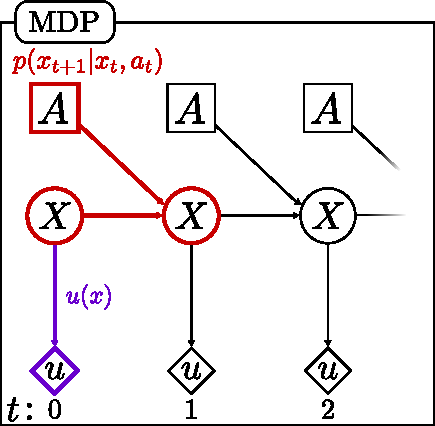
\includegraphics[width=0.45\textwidth]{/home/guillaume/Documents/Thesis/ch2-Background/Figures/mdp3.pdf}}
  \subfigure[on-policy]{\label{fig:mdp_on}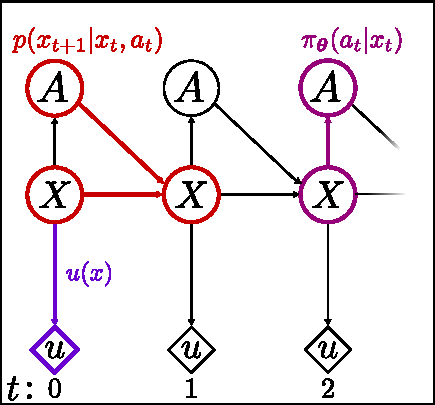
\includegraphics[width=0.45\textwidth]{/home/guillaume/Documents/Thesis/ch2-Background/Figures/mdp2.pdf}} 
  \caption{Dynamical Bayesian Network of a Markov Decision Process; it encodes the temporal relation between the random variables (circles),
  utilities (diamond) and decisions (squares). The arrows specify conditional distributions. In \textbf{(a)} the decision nodes are not considered 
  random variables whilst in \textbf{(b)} they are. From these two DBN  we can read off two conditional distributions, the state transition distribution (in red) and the action distribution (in purple). }
    \label{fig:mdp}
\end{figure}

Solving a MDP means finding a policy whose actions in any given state will always maximise the expected utility. Such 
a policy is usually denoted as $\pi^*$, the optimal policy. As in decision theory, the expected utility is the utility 
of  a sequence of states $u(x_{0:T})$ weighted by its probability . The graphical representation allows to read off directly the probability 
of a sequence of state transitions and actions $(x_{0:T},a_{0:T-1})$, Equation \ref{eq:joint_state_actions}.
\begin{align}\label{eq:joint_state_actions}
  p(x_{0:T},a_{0:T-1}) &= p(x_{0}) \prod_{t=0}^{T-1} p(x_{t+1}|x_t,a_t) \\
  u(x_{0:T}) 	       &= r(x_0) + \gamma r(x_1) + \dots + \gamma^{T-1} r(x_{T-1})  + \gamma^T r(x_T)
\end{align}
We are interested in finding the sequence of action, $a_{0:T}$, which will maximise the expected utility function:
\begin{equation}\label{eq:temporal_expected_utility}
 \argmax_{a_{0:T-1}} U(x_{0:T},a_{0:T-1}) = \max_{a_0} \sum\limits_{x_1}   \cdots  \max_{a_{T-1}} \sum\limits_{x_T} \Bigg( p(x_{0:T},a_{0:T-1}) u(x_{0:T}) \Bigg)
\end{equation}
Solving the above directly in its current form would have an exponential complexity. By making use of the first order 
markov assumption and that current rewards do not dependent future rewards, the sums in Equation \label{eq:max_util} can be re-arranged and 
and recursive patter will emerge which we can take advantage off. Lets start from the last time step and move out of the sum all elements 
which do not depend on $T$ and $T-1$, which results in Equation \ref{eq:expansion}
\begin{align}\label{eq:expansion}
 &\argmax_{a_{0:T-1}} U(x_{0:T},a_{0:T-1}) =\max_{a_0} \sum\limits_{x_1}   \cdots  \max_{a_{T-2}} \sum\limits_{x_{T-1}}  \nonumber\\
 &p(x_{0:T-1},a_{0:T-2})  \left( u(x_{0:T-2}) + \gamma^{T-1} \left( r(x_{T-1}) +  \gamma \max_{a_{T-1}} \sum\limits_{x_{T}} p(x_{T}|x_{T-1},a_{T-1}) r(x_{T}) \right) \right)
\end{align}
From the rearrangement we notice that Equation \ref{eq:expansion} has the same functional form as Equation \ref{eq:temporal_expected_utility}, 
except that the recursive component can be summarised by Equation \ref{eq:bellman}, which is known as 
the \textbf{Bellman} optimal equation.
\begin{equation}\label{eq:bellman}
 V^*(x_t) := r(x_t) + \gamma \max_{a_t} \sum\limits_{x_{t+1}} p(x_{t+1}|x_t,a_t) V(x_{t+1})
\end{equation}
For the terminal state $V_T(x_T) = r(x_T)$. The bellman equation is a means of solving a sequential decision problem 
through use of dynamic programming. It says the the utility of the current state is based on the immediate reward and 
the discounted maximum utility of the next state. Making use of this recursion reduced the computation complexity is 
quadratic in the number of states, $\BigO(T\, |A|\, |X|^2)$. To find the optimal value and subsequent policy an approach 
would be to repeatedly apply the bellman equation to each state until the value function converges. What makes the problem 
hard to solve is maximisation over the actions. This induces two problems, the first is that the optimisation is nonlinear 
and the second is that if the action space is continuous the maximisation will be expensive to compute.
This brings use to the two main approaches to solving a the MDP process: \textbf{off-policy} and \textbf{on-policy}.
Off-policy methods solve directly for the optimal value function $V^*(x)$ and perform the maximisation over the actions, \textbf{Value-Iteration (VI)}
is such a method. On-policy approaches find the optimal value and policy through repeating \textbf{policy evaluation} and
\textbf{improvement} steps. In the policy evaluation the value or utility of a policy is found through solving the on-policy version of the Bellman 
equation:
\begin{equation}\label{eq:on_policy_bellman}
  V^{\pi}(x_t) := r(x_t) + \gamma \sum\limits_{a_t} \policy(a_t|x_t) \sum\limits_{x_{t+1}} p(x_{t+1}|x_t,a_t) V(x_{t+1})
\end{equation}
In the policy improvement step the policy is made more greedy by maximising the value function. Through the repetition of these two 
steps both the value function and policy converge to the optimal. On-policy methods are preferred in settings where the action 
space is highly continuous, such as in robotics. Using dynamic programming is however not the method of choice since it requires 
multiple passes through the entire state space and for this it is necessary to have the model of the state transition a priori. 
Instead \textbf{Reinforcement Learning (RL)} methods are used to find an optimal value and policy. RL is a sample based approach
in which an agent interacts with the environment gathering examples of state transitions and rewards (the utility) and uses them 
to gradually solve the bellman equation.

We introduced the formulation of a sequential decision process in the form of a MDP model and showed how an optimal policy 
and value function are obtained through maximising the expected utility. The re-arrangement of the sums via
variable elimination allows to take advantage of a recursive structure present in the markov chain. The recursive component 
turns out to be the Bellman optimal equation, which when solved (via dynamic programming or reinforcement learning) results 
in an optimal value and policy function. A MDP models the uncertainty inherent in the state transition but not the uncertainty 
of the state. The MDP assumes that the state space is always fully observable, which is a strong assumption. In robotics the 
on bored sensors return an estimate of the state with a certain amount of uncertainty associated with it. To take this additional
uncertainty into consideration the MDP has to accommodate it. This leads to a Partially Observable Markov Decision Process (POMDP).

%The problems in robotics are solved with \textbf{Reinforcement Learning (RL)} which is set of sample based 
%methods for solving both Equation \ref{eq:bellman} and \ref{eq:on_policy_bellman}, instead of using dynamic programming methods like VI.
%The reason is that the state transition function (dynamic model) is not known a priori.
% a two step approach, first an initial policy is assumed at disposition and the 
% value function of this policy is evaluated, a step known as .
% To find the first optimal action we have to consider the expected utility for all $N$ states and take the action which has the highest value,
%\begin{equation}\label{eq:max_util}
%  U(a_0|x_0) =  \cdots \max_{a_{T-2}} \sum\limits_{x_{T-1}} \max_{a_{T-1}}  \sum\limits_{x_T}  \prod_{t=0}^{T-1} p(x_{t+1}|x_t,a_t) u(x_{1:T})
%end{equation}
%Before going into how to solve a temporal decision problem, we have to introduce a way of representing it. 
%A typical representation is done with a graphical model. Graphical models allow to represent . There are many different types of graphical models and we will be considering Directed Acyclic Graphs (DAC) and 
%when considering an continuous reoccurring decision process DACs are referred to as \textbf{Dynamic Bayesian Networks (DBN)}.
%We are manly interested in DBNs because they are predominantly used in robotics and AI for solving infinite-horizon decision problems.
%In Figure \ref{fig:mdp} we illustrate a DBN of a sequential decision problem where the arrows encode conditional distributions. For instance the state 
%space random variable node, $X$, has two children $A$ and itself $X$ at a previous time step, this connection reads as $p(x_{t+1}|x_t,a_t)$. 
%The decision and utility nodes are not considered random variables in the left subfigure.


% which allow to illustrate infinite-horizon stationary decision processes among others. These types of DAC graphs are also called 
% If the decision problem had a fixed horizon it could be illustrated by an \textbf{influence diagrams}. 
% Influence diagrams are for finite temporal decision process (also called finite-horizon) whilst DBNs are for infinite continuously recurring sequential decisions.
% In Figure \ref{fig:mdp} we illustrate the DBN of a temporal decision problem. 


%Figure \ref{fig:mdp} illustrates the DBN of a first order \textbf{Markov Decision Process (MDP)}.
%An MDP is a \textbf{model} of a temporal decision process which is characterised by the tuple, $(X,A,p(x_{t+1}|x_t,a_t),r(x),\gamma)$, where the models are 
%the state transition function $p(x_{t+1}|x_t,a_t)$ and utility function $r(x)$.



%\subsection{Solving a sequential decision process}

%Lets consider a decision problem of length $T$ in a world which has $N$ states. 
%Given an utility function we first want to find the initial action, $a_0$ which will
%be optimal. 

%This means that the action $a_0$ must maximises the expected utility given all resulting future states and actions. 
%\begin{equation}\label{eq:utility_one}
%  a^*_0 =  \argmax_{a_0}  U(a_0|x_0)
%\end{equation}
%Equation \ref{eq:utility_one}, is the maximisation of the expected utility at time step $0$ given that we are 
%starting in state $i$ and that every following action is optimal (also maximise the expected 
%utility). 

%The utility and associated probability of this utility are given by Equation  \ref{eq:utility_one_var}
%\begin{align}\label{eq:utility_one_var}
%  r(x_{0:T}) 	     &= r(x_0) + \gamma r(x_1) + \gamma^2 r(x_2) + \cdots + \gamma^{T} r(x_T)\\
%  p(x_{0:T},a_{0:T-1}) &= p(x_0) \prod_{t=0}^{T-1} p(x_{t+1}|x_t,a_t)
%\end{align}

% applying the method on a finite-horizon Markov Decision processes is equivalent to Value Iteration where the argmax in each iteration is solved be means of an inference query.
%The first change is to the 
%utility function itself. 
%To be consistent with the literature regarding sequential decision processes, namely 
%work in operational research, AI, optimal control theory and 
%There are two main forms 
%of representing such as decision problem:  in, markov decision processes, partially observable 
%marov decision process. 
% Summary of Bayesian decision Tree CPT table etc..


\subsection{POMDP}

% Define box and box title style
%\tikzstyle{pomdp_box}  = [draw=black, fill=blue!20, very thick,  rectangle, rounded corners, inner sep=10pt, inner ysep=20pt]
%\tikzstyle{fancytitle} = [fill=white,draw= black, text=white,rounded corners=1mm,text=black]

%\begin{figure}[h]
%\centering
%\begin{tikzpicture}
%\node [pomdp_box] (box){%
%    \begin{minipage}{\textwidth}
%      \begin{itemize}
%       \item[] \textbf{States, Actions, Observations} 
      
%      \item[] \textbf{State transition function:} $\mathbf{p(x_{t+1}|x_t,a_t)}$\\ The state transition function models the uncertainty originating from motion noise and is 
%       represented by the conditional probability distribution (or likelihood) function, $p(x_{t+1}|x_t,a_t) \in \mathbb{R}$,
%       which gives the probability of moving to state $x_{t+1}$ given that action $a_t$ was applied in state $x_t$. 
      
%      \item[] \textbf{Observation function}: $\mathbf{p(y_t|x_t)}$\\ The observation function returns the probability 
%       or likelihood of the current observing $y_t$ given a known state $x_t$. It is modelled 
%       by the conditional distribution $p(y_t|x_t) \in \mathbb{R}$.
      
%      \item[] \textbf{Belief:} $\mathbf{b_t(x)}$ \\
%       A belief is probability distributions, $b_t(x)$, over the state space $X$ and quantifies both 
%       motion and observation uncertainty. 
      
%      \item[] \textbf{State space estimator:} $\mathbf{b_t(x) = \tau(b_{t-1}(x),u_{t-1},y_t)}$\\ 
%       Updates a belief given a motion and observation, it makes use of both the motion and observation functions 
%       defined in the POMDP. The state space estimation function, $\tau$, can be any kind of state space filter such as 
%       an Extended Kalman Filter (EKF) or a Particle Filter (PF).
    
%       \item[] \textbf{Reward function:} $\mathbf{R(x_t,u_t)}$\\
%        The reward becomes a function of the belief $R(b_t,u_t)$ which is the expected value of the original reward 
%	function $\mathbb{E}_{x_t \sim b_t}[R(x_t,u_t)]$.
%       \item[] \textbf{Discount factor} $\gamma \in [0,1]$;
%      \end{itemize}
%    \end{minipage}
%};
%\node[fancytitle, right=10pt] at (box.north west) {(PO)MDP \& \textit{belief}-MDP};
%\end{tikzpicture}%
%\caption{Description of the individual elements necessary to formalise a POMDP and a \textit{belief}-MDP.}
%\label{fig:pomdp_tik}
%\end{figure}

A POMDP is a popular approach for formulating a decision making process under both motion and measurement uncertainty;
In Figure \ref{fig:pomdp_tik} we describe all of the components necessary for a POMDP.

Since the states are not observable, the agent cannot choose its actions based on the state. The explicit 
representation of the past events is typically memory expensive. Instead it is possible to summarize all relevant 
information from previous actions and observations in a probability distribution over the state space, known as the
belief state. 

\begin{figure}[h]
 \centering
 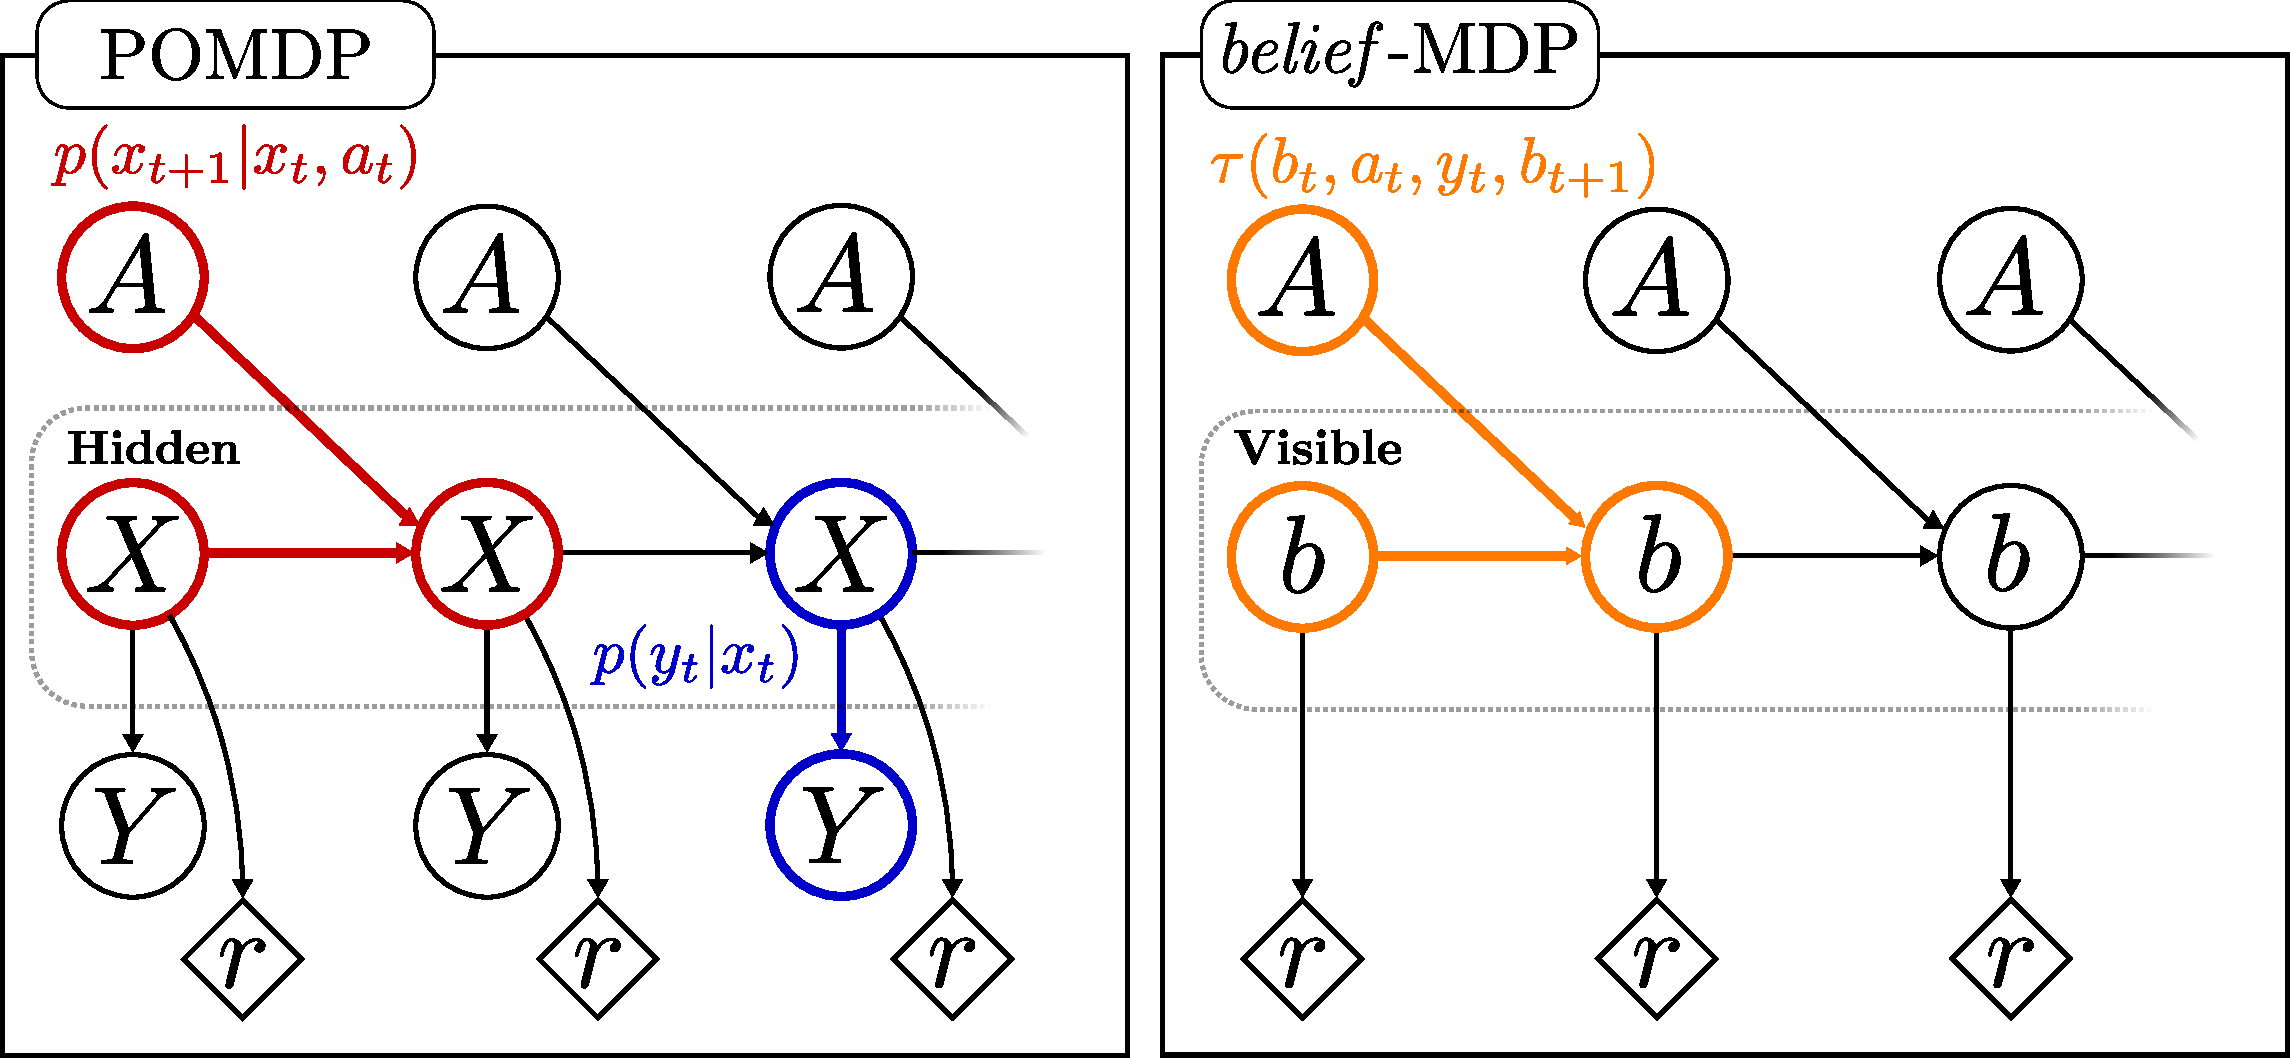
\includegraphics[width=\textwidth]{/home/guillaume/Documents/Thesis/ch2-Background/Figures/pomdp.pdf}
  \caption{ad}
\end{figure}


Because the state space is partially observable the expected reward has to be computed for each possible history of states, actions and observations.
All approaches in the literature instead encapsulate all these possible histories into a belief state $b(x_t)$ which is a 
probability distribution (referred to in the POMDP literature as an information state, \textit{I}-state) over the state space $x_t$ and use this 
new state description to cast the POMDP into a \textit{belief}-MDP (states are probability distributions, beliefs). 

The new description of the problem is now in terms of belief space $<\mathcal{B},U,\tau,R,\gamma>$ where $\mathcal{B}$ is the set of 
all possible beliefs and 
The reward becomes a function of the belief $R(b_t,u_t)$ which is the expected value of the original reward 
function $\mathbb{E}_{x_t \sim b_t}[R(x_t,u_t)]$, The goal is to find an optimal action for each belief such that 
the policy $\pi(b_t,u_t)$ maximises the expected reward, Equation \ref{eq:optimal_value_f}.

\begin{align}\label{eq:optimal_value_f}
% V^{\pi^*}(b_{t-1}) &= \mathbb{E}\left[\sum\limits_{t=0}^{\infty} \gamma^{t} R(x_t,u_t) \bigg| \pi,b_{t-1}\right]\\
 V^{\pi^*}(b_{t-1}) &= \max_{u_{t-1}} \bigg[ R(b_{t-1},u_{t-1}) + \gamma \cdot \mathbb{E}_{y_t}\left[ V^{\pi}(b_t)  \right] \bigg]
\end{align}

From considering the decision belief tree of the POMDP, Figure \ref{fig:pomdp_bel_tree}, we can appreciate the complexity of the problem
of finding an optimal policy. Given a discrete set of actions and observations to update the belief $b_1$ we have to consider a time 
complexity of $\mathcal{O}(|U||Y|^T)$ where $T$ is the depth of the tree (the planning horizon). Given that we have a finite set of 
belief the complexity solving the POMDP is $\mathcal{O}(|\mathcal{B}||U||Y|^T)$. 


\begin{figure}[h]
 \centering
 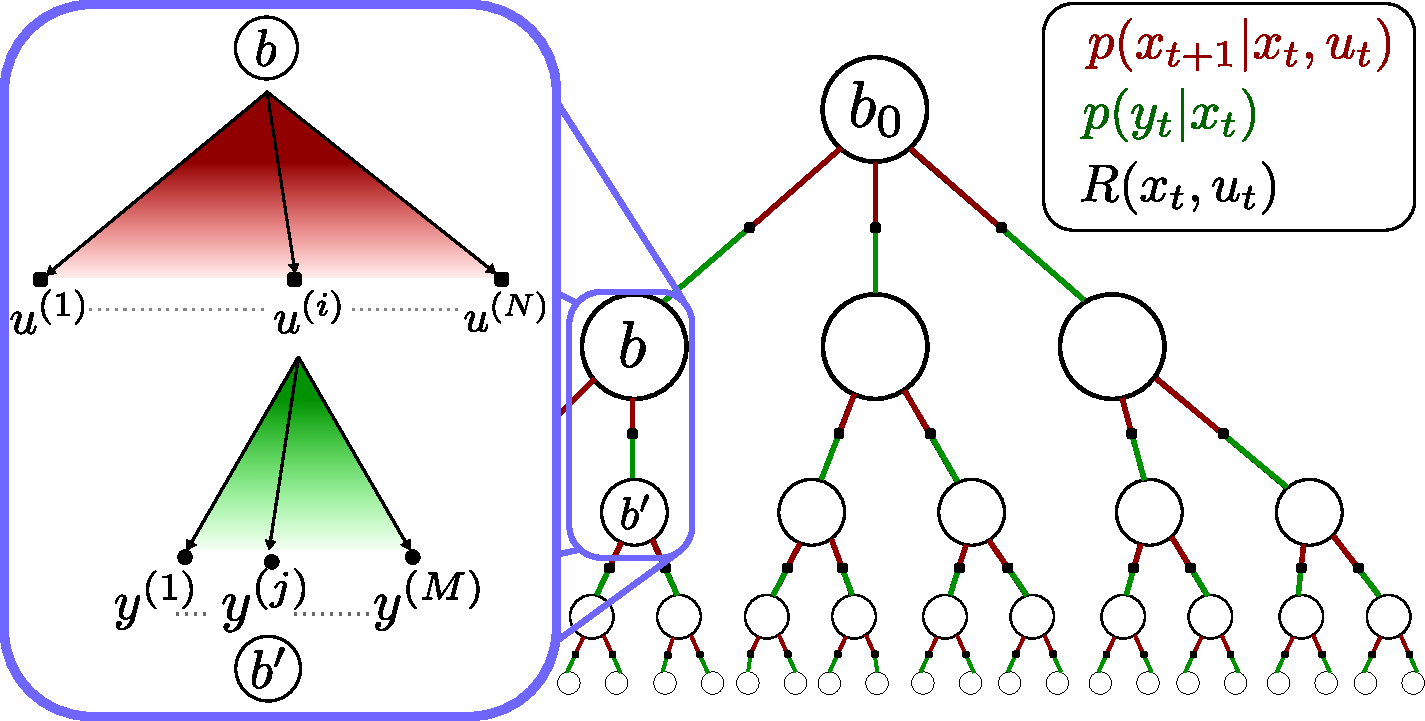
\includegraphics[width=\textwidth]{/home/guillaume/Documents/Thesis/ch2-Background/Figures/belief_tree.pdf}
  \caption{ad}
\end{figure}


\section{State of the art}

%\begin{figure}[h]
% \centering
% 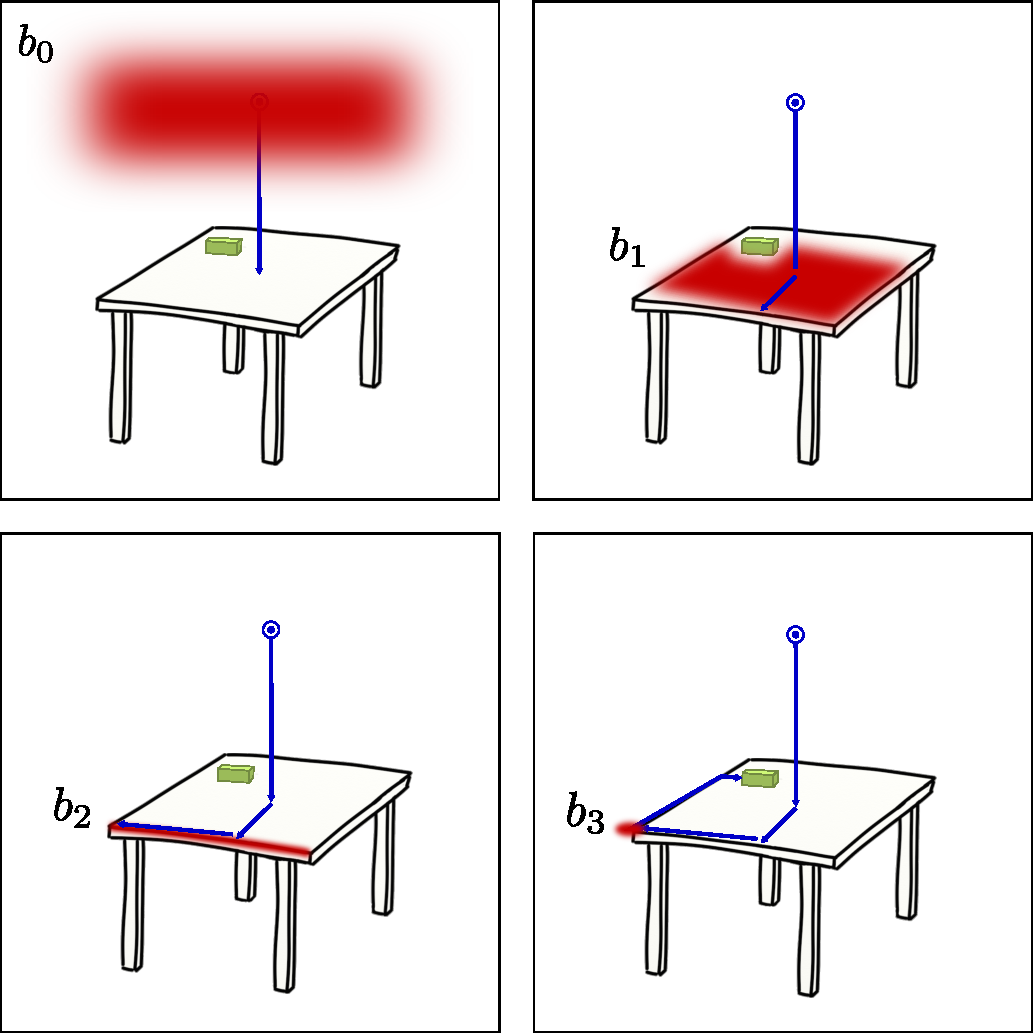
\includegraphics[width=\textwidth]{/home/guillaume/Documents/Thesis/ch2-Background/Figures/reasoning_uncertainty_concept1.pdf}
% \caption{ad}
%\end{figure}

% Standard decision theory, (no temporal aspect taken into consideration)
% Markov decision process (MDP).


% 1) POMDP
%	Based on Markove Decision Process
%	Talk about background in Optimal control and decision theor
%	Assume convex cost function, can be in feature space
%	 1.1) Approximatee POMDP
%	 1.2) MC-POMDP


% 2) Belief space (planning)
%	belief roadmap (assumption on the noise)
%
% 3)  Belief space (optimal control)
%
%
% 4) Assumptions about motion noise and observation 
%
%

% Policy search
\cite{Sol_POMDP_Policy_space_1998}

\subsubsection{Tree search}

\subsubsection{Planning}
$b = (\mu,\Sigma)$
\cite{Quadrator_2008},\cite{BelRoadMap_2009}


\subsubsection{Optimal control}
$b = (\mu,\Sigma)$
 
\cite{Erez10ascalable},
\cite{mc_update_ppomdps}, 
\cite{Platt-RSS-10}

 
% Continous

Optimal control methods represent the belief by a Gaussian function 


\cite{Bayesian_explor_exploit_2009},\cite{Spaan05icra},\cite{Thrun_2005}
 
% Sample based replanning

\cite{Rand_belief_space_replanning}
 
 
 % Online vs Offline methods
 \cite{Ross08onlineplanning}
 
 % Macro-Actions
 \cite{Macro_uncertainty_2011}

\section{Summary}




